% !TEX spellckeck=en_GB

\section{Recurrent Neural Networks}\label{sec:rnn}

The recurrent neural network (RNN) models a unit that has "memory". The memory is encoded as a state variable, and is ordinarily concatenated with the input to make a prediction. The model predictions typically enact a sequence which has led to applications text generation, time-series predictions, and other serialized applications. RNNs were first discussed in a theoretical paper by Jordan, MI in 86' but implemented in the modern temporal sense by \citet{Pearlmutter1989}. A simple graphical representation of the RNN cell is presented in figure \ref{fig:rnn}

\begin{figure}[h]
\centering
\tikzset{every picture/.style={line width=0.75pt}} %set default line width to 0.75pt        


\tikzset{every picture/.style={line width=0.75pt}} %set default line width to 0.75pt        

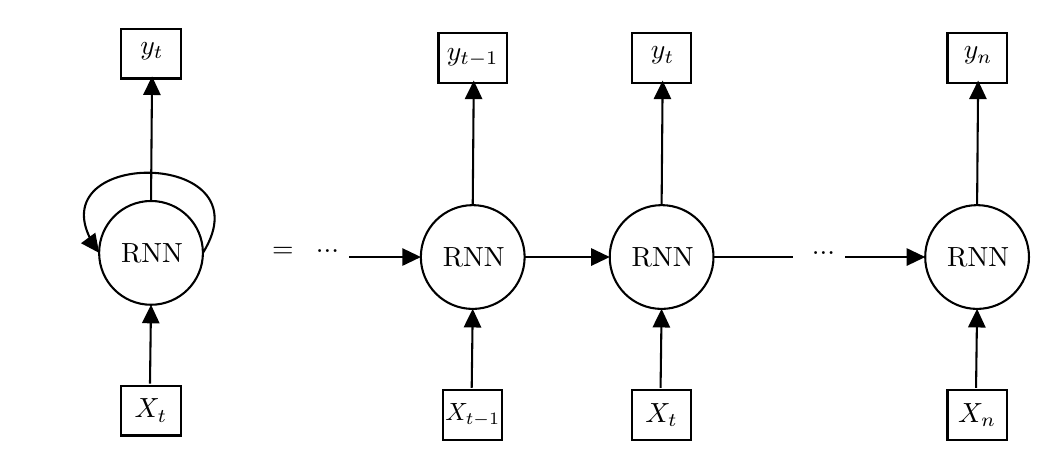
\begin{tikzpicture}[x=0.75pt,y=0.75pt,yscale=-1,xscale=1]
%uncomment if require: \path (0,300); %set diagram left start at 0, and has height of 300

%Shape: Circle [id:dp8533848553232608] 
\draw   (79,153) .. controls (79,139.19) and (90.19,128) .. (104,128) .. controls (117.81,128) and (129,139.19) .. (129,153) .. controls (129,166.81) and (117.81,178) .. (104,178) .. controls (90.19,178) and (79,166.81) .. (79,153) -- cycle ;
%Shape: Rectangle [id:dp3356851682550741] 
\draw   (89.75,217) -- (118.25,217) -- (118.25,241) -- (89.75,241) -- cycle ;
%Shape: Rectangle [id:dp015360643602005286] 
\draw   (89.75,45) -- (118.25,45) -- (118.25,69) -- (89.75,69) -- cycle ;
%Curve Lines [id:da13241738005580928] 
\draw    (77.42,150.74) .. controls (45.07,101.98) and (161.01,101.78) .. (129,153) ;

\draw [shift={(79,153)}, rotate = 233.67] [fill={rgb, 255:red, 0; green, 0; blue, 0 }  ][line width=0.75]  [draw opacity=0] (8.93,-4.29) -- (0,0) -- (8.93,4.29) -- cycle    ;
%Straight Lines [id:da8737873439903896] 
\draw    (103.97,180) -- (103.5,216) ;

\draw [shift={(104,178)}, rotate = 90.75] [fill={rgb, 255:red, 0; green, 0; blue, 0 }  ][line width=0.75]  [draw opacity=0] (8.93,-4.29) -- (0,0) -- (8.93,4.29) -- cycle    ;
%Straight Lines [id:da7493250835057881] 
\draw    (104.48,70) -- (104,128) ;

\draw [shift={(104.5,68)}, rotate = 90.48] [fill={rgb, 255:red, 0; green, 0; blue, 0 }  ][line width=0.75]  [draw opacity=0] (8.93,-4.29) -- (0,0) -- (8.93,4.29) -- cycle    ;
%Shape: Circle [id:dp35751159267212573] 
\draw   (234,155) .. controls (234,141.19) and (245.19,130) .. (259,130) .. controls (272.81,130) and (284,141.19) .. (284,155) .. controls (284,168.81) and (272.81,180) .. (259,180) .. controls (245.19,180) and (234,168.81) .. (234,155) -- cycle ;
%Shape: Rectangle [id:dp2991223335771349] 
\draw   (244.75,219) -- (273.25,219) -- (273.25,243) -- (244.75,243) -- cycle ;
%Shape: Rectangle [id:dp26798597888426934] 
\draw   (242.5,47) -- (275.5,47) -- (275.5,71) -- (242.5,71) -- cycle ;
%Straight Lines [id:da9184227308196455] 
\draw    (258.97,182) -- (258.5,218) ;

\draw [shift={(259,180)}, rotate = 90.75] [fill={rgb, 255:red, 0; green, 0; blue, 0 }  ][line width=0.75]  [draw opacity=0] (8.93,-4.29) -- (0,0) -- (8.93,4.29) -- cycle    ;
%Straight Lines [id:da22975840892719268] 
\draw    (259.48,72) -- (259,130) ;

\draw [shift={(259.5,70)}, rotate = 90.48] [fill={rgb, 255:red, 0; green, 0; blue, 0 }  ][line width=0.75]  [draw opacity=0] (8.93,-4.29) -- (0,0) -- (8.93,4.29) -- cycle    ;
%Shape: Circle [id:dp9315127897645317] 
\draw   (325,155) .. controls (325,141.19) and (336.19,130) .. (350,130) .. controls (363.81,130) and (375,141.19) .. (375,155) .. controls (375,168.81) and (363.81,180) .. (350,180) .. controls (336.19,180) and (325,168.81) .. (325,155) -- cycle ;
%Shape: Rectangle [id:dp6992764849342432] 
\draw   (335.75,219) -- (364.25,219) -- (364.25,243) -- (335.75,243) -- cycle ;
%Shape: Rectangle [id:dp9244658583151169] 
\draw   (335.75,47) -- (364.25,47) -- (364.25,71) -- (335.75,71) -- cycle ;
%Straight Lines [id:da013335644895819732] 
\draw    (349.97,182) -- (349.5,218) ;

\draw [shift={(350,180)}, rotate = 90.75] [fill={rgb, 255:red, 0; green, 0; blue, 0 }  ][line width=0.75]  [draw opacity=0] (8.93,-4.29) -- (0,0) -- (8.93,4.29) -- cycle    ;
%Straight Lines [id:da47760247146100654] 
\draw    (350.48,72) -- (350,130) ;

\draw [shift={(350.5,70)}, rotate = 90.48] [fill={rgb, 255:red, 0; green, 0; blue, 0 }  ][line width=0.75]  [draw opacity=0] (8.93,-4.29) -- (0,0) -- (8.93,4.29) -- cycle    ;
%Straight Lines [id:da7862918954109384] 
\draw    (284,155) -- (323,155) ;
\draw [shift={(325,155)}, rotate = 180] [fill={rgb, 255:red, 0; green, 0; blue, 0 }  ][line width=0.75]  [draw opacity=0] (8.93,-4.29) -- (0,0) -- (8.93,4.29) -- cycle    ;

%Shape: Circle [id:dp5561688511939951] 
\draw   (477,155) .. controls (477,141.19) and (488.19,130) .. (502,130) .. controls (515.81,130) and (527,141.19) .. (527,155) .. controls (527,168.81) and (515.81,180) .. (502,180) .. controls (488.19,180) and (477,168.81) .. (477,155) -- cycle ;
%Shape: Rectangle [id:dp3227398330747131] 
\draw   (487.75,219) -- (516.25,219) -- (516.25,243) -- (487.75,243) -- cycle ;
%Shape: Rectangle [id:dp040272455053374845] 
\draw   (487.75,47) -- (516.25,47) -- (516.25,71) -- (487.75,71) -- cycle ;
%Straight Lines [id:da6201233594039455] 
\draw    (501.97,182) -- (501.5,218) ;

\draw [shift={(502,180)}, rotate = 90.75] [fill={rgb, 255:red, 0; green, 0; blue, 0 }  ][line width=0.75]  [draw opacity=0] (8.93,-4.29) -- (0,0) -- (8.93,4.29) -- cycle    ;
%Straight Lines [id:da35639259950390456] 
\draw    (502.48,72) -- (502,130) ;

\draw [shift={(502.5,70)}, rotate = 90.48] [fill={rgb, 255:red, 0; green, 0; blue, 0 }  ][line width=0.75]  [draw opacity=0] (8.93,-4.29) -- (0,0) -- (8.93,4.29) -- cycle    ;
%Straight Lines [id:da7814656791881325] 
\draw    (375,155) -- (413.5,155) ;


%Straight Lines [id:da5961879457049848] 
\draw    (438.5,155) -- (475,155) ;
\draw [shift={(477,155)}, rotate = 180] [fill={rgb, 255:red, 0; green, 0; blue, 0 }  ][line width=0.75]  [draw opacity=0] (8.93,-4.29) -- (0,0) -- (8.93,4.29) -- cycle    ;

%Straight Lines [id:da20737537017177732] 
\draw    (199.5,155) -- (232,155) ;
\draw [shift={(234,155)}, rotate = 180] [fill={rgb, 255:red, 0; green, 0; blue, 0 }  ][line width=0.75]  [draw opacity=0] (8.93,-4.29) -- (0,0) -- (8.93,4.29) -- cycle    ;


% Text Node
\draw (104,229) node   {$X_{t}$};
% Text Node
\draw (104.5,56) node   {$y_{t}$};
% Text Node
\draw (104.5,153) node  [align=left] {RNN};
% Text Node
\draw (167.5,153) node   {$=$};
% Text Node
\draw (259,231) node [scale=0.9]  {$X_{t-1}$};
% Text Node
\draw (259,59) node   {$y_{t-1}$};
% Text Node
\draw (259.5,155) node  [align=left] {RNN};
% Text Node
\draw (350,231) node   {$X_{t}$};
% Text Node
\draw (350.5,58) node   {$y_{t}$};
% Text Node
\draw (350.5,155) node  [align=left] {RNN};
% Text Node
\draw (502,231) node   {$X_{n}$};
% Text Node
\draw (502.5,58) node   {$y_{n}$};
% Text Node
\draw (502.5,155) node  [align=left] {RNN};
% Text Node
\draw (428,153) node   {$...$};
% Text Node
\draw (189,152) node   {$...$};


\end{tikzpicture}

\caption[Recurrent neural network cell]{A graphical illustration of the RNN cell. The self-connected edge in the left-hand side denotes the temporal nature we unroll on the right side. The cell takes as input a state vector and an input vector at time t and outputs a prediction and the new state vector used for the next prediction. Internally the simplest form this operation takes is to concatenate the state vector with the input and use an ordinary dense network as described in section \ref{sec:ANN} trained with back-propagation.}\label{fig:rnn}
\end{figure}

The memory encoded by the RNN cell is encoded as a state variable. Figure \ref{fig:rnn} gives a good intuition for an RNN cell, but we will elaborate on this by introducing the surprisingly simple forward pass structure for ordinary RNN cells. Let $X_t$ be the input to the RNN cell at time-step from zero to $n$, $\{0 \leq t \leq n: t \in \mathcal{Z} \}$ and $h_t$ be the state of the RNN cell at time $t$. Let also $y_t$ be the output of the RNN at time $t$. The nature of $X$ and $y$ are problem-specific, but common uses of these networks have been the prediction of words in a sentence. Where $X$ would represent the previous word in the sentence and $y$ the prediction over the set of available words for which comes next. An RNN cell can then be concisely formulated as

\begin{align}\label{eq:rnn}
\inner{[X_t, h_t]}{W} + b = h_{t+1},
\end{align}

\noindent where the weight matrix $W$ and bias vector $b$ are defined in the usual manner. Looking back at figure \ref{fig:rnn} the output should be a vector in $y$ space, and yet we have noted the output, $h_t$, as being in the state space of the cell. This notational difference is simply a convenience lending flexibility to our implementation, $h_t$ is transformed to the $y$ space by use of a regular fully connected layer. This transformation is a common trick in machine learning: leaving the inner parts of the algorithm extremely problem agnostic and using end-point layers to fit the problem at hand. To further clarify, we show the forward pass for a simple one-cell RNN in algorithm \ref{algo:rnn}. Expanding from a single cell to a model of complex systems, one can use the output from one RNN cell, $h_{t+1}$, as the input to another producing a deep recurrent network. 

\begin{algorithm}[H]
\SetAlgoLined
\caption{Defining the forward pass of a simple one cell RNN network. The cell accepts the previous state and corresponding data-point as input. These are batched vectors both, and so one usually concatenates the vectors along the feature axis to save time when doing the matrix multiplication. The cell maintains a weight matrix, $\boldsymbol{W}$, and bias, $b$, which will be updated by back-propagation of errors in the standard way.}\label{algo:rnn}
\KwResult{$\boldsymbol{h}_{t+1}$}
\KwIn{$\boldsymbol{h}_t$, $\boldsymbol{X}_t$}
\KwData{$\boldsymbol{W}$, b}
$\boldsymbol{F} \gets$ \KwSty{concatenate}(($h_t$, $\boldsymbol{X}_t$), axis$=1$)\;
$\boldsymbol{h}_{t+1}$ $\gets$ \KwSty{matmul}($\boldsymbol{F}$, $\boldsymbol{W}$) + b\;
\KwRet{$\boldsymbol{h}_{t+1}$}
\end{algorithm}

\noindent When designing a neural network, the researcher principally has five basic choices regarding the sequentiality of the model. We represent these five in figure \ref{fig:ann_architectures}.

\begin{figure}
\centering
\includegraphics[width=\textwidth]{../figures/ann_types}
\caption[Archetypes of recurrent neural architectures]{The advent of recurrent networks enabled machine learning researchers to both model complex sequential behaviours like understanding patterns in a corpus of texts as well as using sequences to predict a single multivariate outcome and more. The leftmost figure \textbf{1)} represents an ordinary neural network, where the rectangles are matrix objects, red for input, blue for output and green for intermediary representations and the arrows are matrix operations like concatenation, multiplication and other arithmetic. \textbf{2)} shows a recurrent architecture for sequence output e.g. image captioning. Where the information about the previous word gets passed along forward by the state of the previous cell. \textbf{3)} transforming a sequence of observations to a single multivariate outcome. The classic example of which is sentiment prediction from text data. \textbf{4), 5)} Sequenced input and output can either be aligned as in the latter or misaligned as in the former. An example of a synced sequence to sequence can be phase prediction from a time series of a thermodynamic system. Un-synced applications include machine translation where sentences are processed then output in another language. Figure copied from \cite{Karpathy2015}}\label{fig:ann_architectures}
\end{figure}

\subsection{Long short-term memory cells}\label{sec:lstm}

One of the principal challenges for the RNN cell is in the handling of the state of the cell. The state acts as a sort of memory, but without moderation, it tries to recall the entire history of the sequence. \citet{Hochreiter1997} proposed a solution to this problem in their description of the long short-term memory (LSTM) network. The LSTM network introduced the ability for the network to selectively forget part of its memory. Being able to forget parts of the history was a boon to the language processing community, as they regularly tackle problems with both long and short term relationships. 

The LSTM network implements a series of layers inside each cell. By combining sigmoid, $\sigma{\cdot}$, and the hyperbolic tangent function, $\tau(\cdot)$, they compute point-wise manipulations of the state $\boldsymbol{h}_t$, previous output $\boldsymbol{c}_t$ and input $\boldsymbol{x}_t$. Lastly, we define the input gate $\boldsymbol{i}_t$, output gate $\boldsymbol{o}_t$ and forget gate $\boldsymbol{f}_t$, each with their own weight matrices $\boldsymbol{W}_{\{i, f, o, c\}}$. The gates are computed as

\begin{align}
\boldsymbol{i_t} = \sigma(\boldsymbol{W}_i[\boldsymbol{h}_{t-1}, \boldsymbol{x}_t]),\\
\boldsymbol{f_t} = \sigma(\boldsymbol{W}_f[\boldsymbol{h}_{t-1}, \boldsymbol{x}_t]),\\
\boldsymbol{o_t} = \sigma(\boldsymbol{W}_o[\boldsymbol{h}_{t-1}, \boldsymbol{x}_t]).
\end{align}

\noindent Following from these definitions, we can compute the new state and cell outputs

\begin{align}
\hat{\boldsymbol{c}}_t &= \tau (\boldsymbol{W}_o[\boldsymbol{h}_{t-1}, \boldsymbol{x}_t]), \\
\boldsymbol{c}_t &= \boldsymbol{i}_t \circ \hat{\boldsymbol{c}}_t + \boldsymbol{f}_t \circ \boldsymbol{c}_{t-1}, \\ 
\boldsymbol{h}_t &= \boldsymbol{o}_t \circ \tau (\boldsymbol{c}_t).
\end{align}

\noindent Recall the Hadamard product denoted by $\circ$, and the concatenation of two vectors denoted by square brackets. In the equations above, we have also followed the convention of including a column of ones in the data. This inclusion bakes the biases into the weight matrices, and is convenient for notational clarity. 

The LSTM network was designed to allow for the network to forget parts of the input. However, it also solves a vanishing gradient problem as the gradient flows through the network by the cell outputs.
